\documentclass[conference]{IEEEtran}
\IEEEoverridecommandlockouts
% The preceding line is only needed to identify funding in the first footnote. If that is unneeded, please comment it out.
\usepackage[brazil]{babel}
\usepackage{cite}
\usepackage{amsmath,amssymb,amsfonts}
\usepackage{algorithmic}
\usepackage{graphicx}
\usepackage{textcomp}
\usepackage{xcolor}
\def\BibTeX{{\rm B\kern-.05em{\sc i\kern-.025em b}\kern-.08em
    T\kern-.1667em\lower.7ex\hbox{E}\kern-.125emX}}

\begin{document}
%====================================================================================
\title{Relatório de atividade\\ Implementação de Controle \textit{Go-to-Goal} para Robôs com tração diferencial Usando Critério de Estabilidade de Lyapunov }

\author{\IEEEauthorblockN{Matheus Lucas Tavares de Farias}
\IEEEauthorblockA{Prof. AMN Lima \\
Automação Inteligente\\
24 de Julho de 2025
}}

\maketitle

\begin{abstract}
Este relatório descreve a implementação e a análise de duas leis de controle para um robô de tração diferencial com comportamento do tipo \textit{go-to-goal}, ambas baseadas no critério de estabilidade de Lyapunov. O objetivo é conduzir o robô a uma posição-alvo garantindo a convergência assintótica por meio de formulações matemáticas estáveis. A implementação foi realizada em ambiente simulado (CoppeliaSim), utilizando o modelo cinemático \textit{unicycle} do robô Pioneer-3DX, com informações de pose obtidas por sensores virtuais. Os resultados obtidos para cada lei de controle são apresentados de forma detalhada e uma comparação qualitativa e quantitativa é realizada, destacando as principais diferenças entre as abordagens.
\end{abstract}


\begin{IEEEkeywords}
Controle baseado em Lyapunov, modelo unicycle, \textit{Go-to-Goal}, CoppeliaSim.
\end{IEEEkeywords}


%===================================================================================
\section{Introdução}

A navegação de robôs móveis autônomos é um dos principais temas da robótica móvel e tem sido amplamente estudada nas últimas décadas. Um dos desafios clássicos nessa área é o controle de veículos com restrições não-holonômicas, como os robôs com cinemática do tipo unicíclo, em tarefas como alcance de pose e seguimento de trajetórias.

A capacidade de controlar robôs com precisão, mesmo sob restrições cinemáticas, é essencial para aplicações reais, como veículos autônomos, drones terrestres, sistemas de vigilância robótica e robôs assistivos. Métodos de controle com garantias de estabilidade, especialmente aqueles baseados na teoria de Lyapunov, são particularmente relevantes por proporcionarem segurança e previsibilidade no comportamento do sistema.

Este relatório aborda o problema do controle de movimento de robôs móveis do tipo unicíclo, com foco em duas abordagens propostas na literatura. A primeira é uma técnica de controle baseada em Lyapunov voltada à estabilização assintótica para o problema de estacionamento em um alvo fixo, conforme apresentada em \cite{b1} por Aicardi \textit{et al.}. A segunda consiste em um controlador comportamental, também fundamentado em Lyapunov, originalmente proposto por Benbouabdallah \textit{et al.}, em \cite{b2} para rastreamento de alvos móveis, mas aqui analisado em sua aplicação ao caso particular de estabilização em alvos fixos.


%===================================================================================
\section{Teoria de Estabilidade de Lyapunov}

A teoria de Lyapunov fornece uma abordagem indireta para verificar a estabilidade de sistemas dinâmicos sem a necessidade de resolver suas equações diferenciais, uma vez que estas podem não possuir solução analítica. A ideia central é a construção de uma função escalar, chamada função de Lyapunov, que atua como uma ferramenta para avaliar essa estabilidade.

Considere um sistema dinâmico da forma:

\begin{equation}
    \dot{x} = f(x),
    \label{eq:Modelo_Dinamico}
\end{equation}

onde $x \in \mathbb{R}^n$ e $f(0) = 0$, ou seja, a origem é um ponto de equilíbrio.

Diz-se que uma função continuamente diferenciável $V: \mathbb{R}^n \to \mathbb{R}$ é uma função de Lyapunov para esse sistema se satisfaz as seguintes condições:

\begin{itemize}
    \item $V(x) > 0$ para todo $x \neq 0$ e $V(0) = 0$ (positividade definida);
    \item $\dot{V}(x) \leq 0$ para todo $x$ (derivada negativa semidefinida).
\end{itemize}

Se essas condições forem satisfeitas, conclui-se que o ponto de equilíbrio $x = 0$ é estável no sentido de Lyapunov. Além disso, se $\dot{V}(x) < 0$ para todo $x \neq 0$, a estabilidade é dita assintótica, ou seja, as trajetórias não apenas permanecem próximas da origem, como também convergem para ela ao longo do tempo.

Esse método é amplamente utilizado na análise de sistemas não lineares, pois permite estabelecer estabilidade com base apenas na estrutura do sistema e em propriedades qualitativas da função $V(x)$.

Usando essa abordagem, o problema de prova de estabilidade se resume a determinar uma função de Lyapunov que satisfaça as condições propostas. Entretanto, essa tarefa apresenta certo desafio, uma vez que não existe um algoritmo universal para construí-la, exigindo um bom conhecimento do funcionamento do sistema em questão.

Apesar disso, para sistemas lineares, existe uma estrutura bem estabelecida que pode, inclusive, servir como ponto de partida para análises em sistemas não lineares. Nestes casos, uma escolha comum é propor uma função de Lyapunov com forma quadrática.

Considerando uma matriz simétrica definida positiva $P \in \mathbb{R}^{n \times n}$, com $P = P^T$, define-se:

\begin{equation}
    V(x) = x^T P x
    \label{eq:Forma_quadratica}
\end{equation}

Essa forma garante que $V(x)$ é positiva definida e que $V(0) = 0$. A verificação da condição $\dot{V}(x) \leq 0$ pode ser conduzida diretamente a partir da dinâmica do sistema, facilitando a análise de estabilidade.

Com base nessa teoria, é possível montar uma lei de controle para sistemas dinâmicos, como no caso do \textit{Go-to-Goal} para modelos cinemáticos do tipo unicíclo, ao se determinar uma lei de controle para uma função de Lyapunov sugerida, de tal forma que esta possua as características necessárias para provar a estabilidade do sistema.

%===================================================================================
\section{Modelo Cinemático do Robô Unicíclo}

O modelo cinemático do robô unicíclo é amplamente utilizado na robótica móvel para representar veículos com duas rodas acionadas (diferenciais) ou uma única roda com capacidade de movimento para frente e rotação. Este modelo descreve o movimento plano do robô com base em sua posição e orientação, considerando as restrições não-holonômicas impostas pelas rodas.

A configuração do robô é representada por um vetor de estado:

\begin{equation}
    q = \begin{bmatrix}
        x \\
        y \\
        \theta
    \end{bmatrix},
\end{equation}

onde $(x, y)$ representa a posição do robô no plano e $\theta$ é o ângulo de orientação em relação ao eixo $x$ global.

As entradas de controle do sistema são a velocidade linear $v$ e a velocidade angular $\omega$, de forma que a cinemática do robô é dada pelas seguintes equações diferenciais:

\begin{equation}
    \begin{cases}
        \dot{x} = v \cos \theta, \\
        \dot{y} = v \sin \theta, \\
        \dot{\theta} = \omega.
    \end{cases}
    \label{eq:uniciclo}
\end{equation}

Este modelo assume que o robô se move sempre na direção de sua orientação $\theta$, ou seja, não possui capacidade de movimento lateral. Essa restrição caracteriza o sistema como não-holonômico.

Dessa forma, o sistema possui uma estrutura semelhante à expressa na Equação ~\ref{eq:Modelo_Dinamico}. O que possibilita utilizar toda a teoria de Lyapunov para o determinar uma lei de controle para a velocidade linear e angular do robô.

%===================================================================================
\section{Problema do Estacionamento}

O problema do estacionamento (\textit{parking problem}) consiste em levar um robô móvel de uma posição inicial arbitrária até uma pose desejada (posição e orientação) no plano. O objetivo é projetar uma lei de controle que garanta que o robô alcance o alvo de forma estável e precisa.

Esse problema é desafiador, pois o modelo unicíclo não pode ser estabilizado por realimentação contínua e estática em coordenadas cartesianas, conforme demonstrado pelo Teorema de Brockett. Como alternativa, utilizam-se abordagens em coordenadas polares ou transformações de estados que viabilizam o uso de técnicas como o método de Lyapunov para garantir a estabilidade global assintótica do sistema.

Nesta seção, o problema do estacionamento será tratado sob a ótica do controle baseado na teoria de Lyapunov, sob duas perspectivas distintas: a primeira, proposta em \cite{b1}, apresenta uma lei de controle desenvolvida especificamente para alvos fixos; a segunda, originalmente proposta em \cite{b2} para rastreamento de alvos móveis, é aqui analisada em sua aplicação ao caso de estabilização em alvos fixos.


%===================================================================================
\subsection{Abordagem de Aicardi \textit{et al.}}

Essa abordagem é apresentada em \cite{b1} e, conforme descrito pelos autores, o primeiro passo para a construção da lei de controle consiste em redefinir os estados utilizados para descrever o sistema (Equação \ref{eq:Modelo_Dinamico}), a fim de aproximar sua formulação àquela apresentada na Seção II.

Essa redefinição busca representar o sistema em termos de variáveis que quantificam a diferença de posição e orientação entre o robô e o alvo. A Figura~\ref{fig:Sistema_Robo_Alvo} ilustra a relação geométrica entre esses elementos.

\begin{figure}[h!]
    \centering
    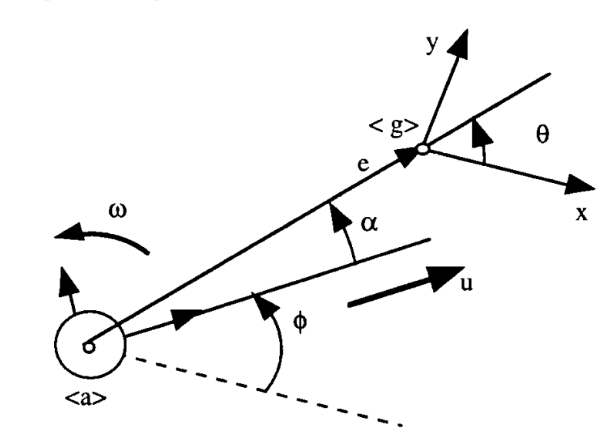
\includegraphics[width=0.4\textwidth]{Figuras/Sistema_Robo_Alvo.png}
    \caption{Sistema Robô-Alvo}
    \label{fig:Sistema_Robo_Alvo}
\end{figure}

A partir dessas considerações, o sistema dinâmico pode ser reescrito como apresentado na Equação \ref{eq:uniciclo_Alt01}.

\begin{equation}
    \begin{cases}
        \dot{e} = -u \cos(\theta - \phi), \\
        \dot{\theta} = \dfrac{u}{e} \sin \alpha, \\
        \dot{\phi} = \omega,
    \end{cases}
    \label{eq:uniciclo_Alt01}
\end{equation}

em que $e$ representa a distância entre o robô e o alvo; $\theta$ é a orientação desejada; $\phi$ é a orientação atual do robô; e $\alpha = \theta - \phi$ representa o erro angular entre a orientação desejada e a atual.

Ao considerar explicitamente $\alpha = \theta - \phi$, é possível reescrever o sistema de forma alternativa, conforme a Equação \ref{eq:uniciclo_Alt02}.

\begin{equation}
    \begin{cases}
        \dot{e} = -u \cos(\alpha), \\
        \dot{\alpha} = -\omega + \dfrac{u}{e} \sin \alpha, \\
        \dot{\theta} = \dfrac{u}{e} \sin \alpha.
    \end{cases}
    \label{eq:uniciclo_Alt02}
\end{equation}

Dessa forma, o sistema é representado no formato da Equação ~\ref{eq:Modelo_Dinamico}, com o vetor de estados definido como $x = [e \quad \alpha \quad \theta]^T$. O ponto de equilíbrio do sistema é dado por $x = [0 \quad 0 \quad 0]^T$, o qual corresponde à condição de estacionamento ideal, o robô posicionado exatamente sobre o alvo e com a mesma orientação.

Contudo, é importante observar que esse ponto constitui uma singularidade no sistema, devido à presença do termo $\dfrac{u}{e} \sin \alpha$, que se torna indefinido quando $e = 0$. Por esse motivo, a estratégia de controle deve garantir que o robô se aproxime desse ponto de forma assintótica, evitando que a distância $e$ se anule em tempo finito, o que invalidaria o modelo.

Com base na representação do sistema dada pela Equação~\ref{eq:uniciclo_Alt02}, já é possível utilizar a teoria de Lyapunov para determinar uma lei de controle que assegure a estabilidade do sistema. O primeiro passo nesse processo é a escolha de uma função de Lyapunov candidata.

Em \cite{b1}, os autores propõem a função definida na Equação ~\ref{eq:Funcao_Lyapunov_1} como candidata à função de Lyapunov:

\begin{equation}
    V = V_1 + V_2 = \frac{1}{2}\lambda e^2 + \frac{1}{2}\left( \alpha^2 + h\theta^2\right), \quad \lambda, h > 0
    \label{eq:Funcao_Lyapunov_1}
\end{equation}

Essa expressão é composta por duas parcelas: $V_1$, associada ao erro de posição do robô em relação ao alvo, e $V_2$, associada ao erro de alinhamento angular entre o robô e o alvo.

Esta função está na forma quadrática. Como discutido na Seção II, esse tipo de função é frequentemente utilizado como ponto de partida para funções de Lyapunov. É possível verificar essa estrutura ao comparar a Equação~\ref{eq:Funcao_Lyapunov_1} com a forma geral quadrática, Equação~\ref{eq:Forma_quadratica}, assumindo-se:

\begin{equation}
    P =
    \begin{bmatrix}
        \dfrac{1}{2}\lambda & 0 & 0\\
        0 & \dfrac{1}{2} & 0\\
        0 & 0 & \dfrac{1}{2}h
    \end{bmatrix},
    x = 
    \begin{bmatrix}
        e\\
        \alpha\\
        \theta
    \end{bmatrix}
    \quad
    \lambda, h > 0
\end{equation}

É fácil verificar que a função $V(x)$ é positiva definida, já que, para $\lambda$ e $h$ positivos, ela é estritamente positiva para todo $x \neq 0$ e nula apenas na origem. Isso satisfaz a primeira condição da teoria de estabilidade de Lyapunov.

Para garantir a estabilidade do sistema, é necessário que a derivada temporal de $V$ seja negativa definida para todo $x \neq 0$. 

Derivando a Equação~\ref{eq:Funcao_Lyapunov_1} no tempo, obtém-se:

\begin{equation}
    \dot{V} = \dot{V}_1 + \dot{V}_2 = \lambda \dot{e} e + \left( \dot{\alpha} \alpha + h\dot{\theta} \theta \right)
    \label{eq:Derivada_Lyapunov_1}
\end{equation}

Substituindo $\dot{e}$, $\dot{\alpha}$ e $\dot{\theta}$ da Equação~\ref{eq:uniciclo_Alt02} na Equação \ref{eq:Derivada_Lyapunov_1}, obtém-se:

\begin{equation}
    \dot{V} = -\lambda e u \cos(\alpha) + \alpha \left[ -\omega + u \dfrac{\sin(\alpha)}{\alpha} \cdot \dfrac{(\alpha + h\theta)}{e} \right]
    \label{eq:Derivada_Lyapunov_1_Comp}
\end{equation}

Nessa expressão, o primeiro termo representa $\dot{V}_1$ e o segundo, $\dot{V}_2$. Ambos serão negativos definidos se as leis de controle $u$ e $\omega$ forem definidas de modo a satisfazer $\dot{V} \leq 0$.

Com base na Equação~\ref{eq:Derivada_Lyapunov_1_Comp}, os autores propõem as seguintes leis de controle:

\begin{equation}
    \begin{cases}
        u = \gamma\cos(\alpha)e, \quad \gamma > 0\\
        \omega = k\alpha + \gamma\dfrac{\sin(\alpha)\cos(\alpha)}{\alpha} (\alpha + h\theta)
    \end{cases}
    \label{eq:Leis_de_controle_1}
\end{equation}

Substituindo essas expressões em $\dot{V}$, obtém-se:

\begin{equation}
    \dot{V} = -\lambda \gamma \cos^2(\alpha) e^2 - k\alpha^2 \leq 0
\end{equation}

Como a derivada de $V$ é negativa definida para todos os estados diferentes da origem, conclui-se, pela teoria de Lyapunov, que o sistema é assintoticamente estável.

%===================================================================================
\subsection{Abordagem de Benbouabdallah \textit{et al.}}

Nesta abordagem, os autores em \cite{b2} propõem uma formulação matemática alternativa para o problema de estacionamento de robôs móveis. Essa formulação considera, como princípio fundamental, o efeito da velocidade do alvo sobre o comportamento do sistema. No entanto, no escopo deste trabalho, assume-se que o alvo encontra-se estacionário no ambiente. Portanto, para os resultados aqui apresentados, a velocidade do alvo será considerada nula.

O desenvolvimento da modelagem inicia-se com a definição de variáveis geométricas fundamentais, representadas na Figura~\ref{fig:Sistema_Robo_Alvo_2}. As equações que descrevem as relações entre essas variáveis são apresentadas a seguir.

\begin{figure}[h!]
    \centering
    \includegraphics[width=0.45\textwidth]{Figuras/Sistema_Robo_Alvo_2.png}
    \caption{Sistema Robô-Alvo}
    \label{fig:Sistema_Robo_Alvo_2}
\end{figure}

As equações de posição, que relacionam a posição do robô e do alvo, são dadas pela Equação~\ref{eq:posicoes}:

\begin{equation}
    \begin{cases}
        D \cos\varphi = x_T - x\\
        D \sin\varphi = y_T - y
    \end{cases}
    \label{eq:posicoes}
\end{equation}

em que $(x, y)$ representa a posição atual do robô no plano cartesiano, enquanto $(x_T, y_T)$ corresponde à posição do alvo. A variável $D$ indica a distância euclidiana entre o robô e o alvo, e $\varphi$ é o ângulo entre a linha que conecta o robô ao alvo e o eixo horizontal.

As relações de orientação são expressas pela Equação~\ref{eq:orientacoes}:

\begin{equation}
    \begin{cases}
        \alpha = \theta - \varphi\\
        \beta = \theta_T - \varphi
    \end{cases}
    \label{eq:orientacoes}
\end{equation}

onde $\theta$ representa o ângulo de orientação atual do robô em relação ao eixo $x$, e $\theta_T$ é o ângulo de orientação desejado ao alcançar o alvo. A variável $\alpha$ representa o ângulo entre a orientação do robô e a linha de visada ao alvo, enquanto $\beta$ é o ângulo entre a orientação desejada e essa mesma linha.

Os erros de controle são definidos na Equação~\ref{eq:erros_controle}:

\begin{equation}
    \begin{cases}
        e_D = D_d - D\\
        e_\alpha = \alpha_d - \alpha
    \end{cases}
    \label{eq:erros_controle}
\end{equation}

em que $D_d$ é a distância desejada entre o robô e o alvo, e $\alpha_d$ é o ângulo desejado entre a orientação do robô e a linha de visada ao alvo. O termo $e_D$ representa o erro de distância, enquanto $e_\alpha$ representa o erro angular.

Essa formulação geométrica fornece as bases para o desenvolvimento das leis de controle que permitirão ao robô alcançar a configuração desejada em relação ao alvo.

A seguir, desenvolve-se o sistema de equações diferenciais que descreve a variação da distância e orientação entre o robô e o alvo, conforme a Equação~\ref{eq:sistema_dinamico}:

\begin{equation}
    \begin{cases}
        \dot{D} = v_T\cos\beta - v\cos\alpha\\
        \dot{\varphi} = \dfrac{v_T}{D}\sin\beta - \dfrac{v}{D}\sin\alpha
    \end{cases}
    \label{eq:sistema_dinamico}
\end{equation}

Para o desenvolvimento da lei de controle, utiliza-se a teoria de Lyapunov. Como sugerido em \cite{b2}, a função candidata de Lyapunov é apresentada na Equação~\ref{eq:Funcao_Lyapunov_2}:

\begin{equation}
    \begin{cases}
        V = V_1 + V_2\\
        V_1 = \dfrac{1}{2}e_D^2\\
        V_2 = \dfrac{1}{2}e_\alpha^2
    \end{cases}
    \label{eq:Funcao_Lyapunov_2}
\end{equation}

Comparando a Equação~\ref{eq:Funcao_Lyapunov_2} com a forma quadrática padrão da Equação~\ref{eq:Forma_quadratica}, observa-se a equivalência ao se considerar:

\begin{equation}
    P =
    \begin{bmatrix}
       \dfrac{1}{2} & 0 \\
       0 & \dfrac{1}{2}
    \end{bmatrix},
    \quad
    x = 
    \begin{bmatrix}
        e_D \\
        e_\alpha
    \end{bmatrix}
    \label{eq:Forma_quadratica_2}
\end{equation}

A função de Lyapunov é, portanto, definida positiva para todo $x \neq 0$ e nula para $x = 0$, satisfazendo a primeira condição do teorema de Lyapunov.

A derivada temporal da função de Lyapunov é dada pela Equação~\ref{eq:Derivada_Lyapunov_2}:

\begin{equation}
    \dot{V} = \dot{V}_1 + \dot{V}_2 = e_D\dot{e}_D + e_\alpha\dot{e}_\alpha
    \label{eq:Derivada_Lyapunov_2}
\end{equation}

Substituindo as derivadas das variáveis de acordo com o sistema dinâmico, obtém-se:

\begin{equation}
    \begin{cases}
        \dot{V}_1 = -e_D \left(v_T\cos\beta - v\cos\alpha\right)\\
        \dot{V}_2 = \alpha\left(w - \dfrac{v_T}{D}\sin\beta + \dfrac{v}{D}\sin\alpha\right)
    \end{cases}
    \label{eq:Derivada_Lyapunov_2_Comp}
\end{equation}

Deseja-se agora encontrar leis de controle para $v$ e $w$ que tornem $\dot{V} \leq 0$. Segundo \cite{b2}, essas leis são dadas pela Equação~\ref{eq:leis_controle_geral}:

\begin{equation}
    \begin{cases}
        v = v_T\dfrac{\cos\beta}{\cos\alpha} - K_v e_D\cos\alpha\\
        w = -K_w\alpha - \dfrac{v}{D}\sin\alpha + \dfrac{v_T}{D}\sin\beta
    \end{cases},
    \quad
    K_v, K_w > 0
    \label{eq:leis_controle_geral}
\end{equation}

Com essa escolha, a derivada de Lyapunov se simplifica para:

\begin{equation}
    \dot{V} = -K_v e_D^2 \cos^2\alpha - K_w \alpha^2 \leq 0
    \label{eq:lyapunov_neg_def}
\end{equation}

Sendo $\dot{V} \leq 0$, a segunda condição do teorema de Lyapunov é satisfeita, garantindo a estabilidade assintótica do sistema.

No escopo deste trabalho, assume-se $v_T = 0$, dado que o alvo está estacionário. Assim, as leis de controle se reduzem à Equação~\ref{eq:leis_controle_final}:

\begin{equation}
    \begin{cases}
        v = -K_v e_D \cos\alpha\\
        w = -K_w \alpha - \dfrac{v}{D} \sin\alpha
    \end{cases},
    \quad
    K_v, K_w > 0
    \label{eq:leis_controle_final}
\end{equation}

%===================================================================================
\section{Resultados}

Após a definição das leis de controle para a velocidade linear e angular do modelo cinemático tipo uniciclo, foi realizada uma simulação no ambiente CoppeliaSim com o objetivo de avaliar sua eficácia na resolução do problema \textit{Go-to-Goal}, utilizando o robô Pioneer 3-DX.

O propósito da simulação foi verificar se as leis de controle, em ambas as abordagens propostas, são capazes de conduzir o robô até o ponto alvo com sucesso.

Para compor as leis de controle das velocidades do robô, foi realizada a medição contínua da posição e da orientação do robô e do alvo ao longo de toda a simulação. Essa medição foi feita por meio de ferramentas fornecidas pelo próprio CoppeliaSim, como as funções \textit{sim.getObjectPosition} e \textit{sim.getObjectOrientation}. A partir dessas grandezas, foi possível calcular os erros de posição e orientação, que são utilizados na formulação das leis de controle.

No entanto, é importante destacar que, no simulador, as velocidades linear e angular do robô não são fornecidas diretamente como entrada. Em vez disso, o controle é feito por meio das velocidades angulares das rodas esquerda e direita do Pioneer 3-DX.

Para contornar essa diferença, foi utilizada a seguinte equação para converter as velocidades desejadas do robô (linear $v$ e angular $w$) nas velocidades angulares das rodas ($\omega_R$ e $\omega_L$):

\begin{equation}
    \begin{cases}
        \omega_R = \dfrac{2v + wL}{2R} \\
        \omega_L = \dfrac{2v - wL}{2R}
    \end{cases}
\end{equation}

Nessa equação, $L$ representa a metade da distância entre as rodas (meio-eixo), $R$ é o raio das rodas, e $\omega_R$ e $\omega_L$ são as velocidades angulares das rodas direita e esquerda, respectivamente.

Com as variáveis de controle devidamente convertidas, foi possível realizar a simulação de um cenário de teste. As trajetórias geradas por cada abordagem foram analisadas, assim como as demais grandezas pertinentes, permitindo avaliar a eficácia das leis de controle na condução do robô até o destino final.


%===================================================================================
\subsection{Cenário de Teste}

O cenário de teste proposto para verificar a eficácia do controle é composto por três cenas distintas, conforme ilustrado nas Figuras~\ref{fig:Cena_teste_1}, \ref{fig:Cena_teste_2},  \ref{fig:Cena_teste_3} e  \ref{fig:Cena_teste_4}.

\begin{figure}[h!]
    \centering
    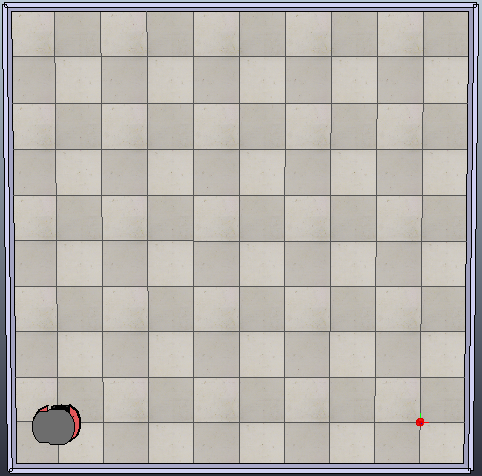
\includegraphics[width=0.3\textwidth]{Figuras/Cena_teste_1.png}
    \caption{Cena de teste 1}
    \label{fig:Cena_teste_1}
\end{figure}

\begin{figure}[h!]
    \centering
    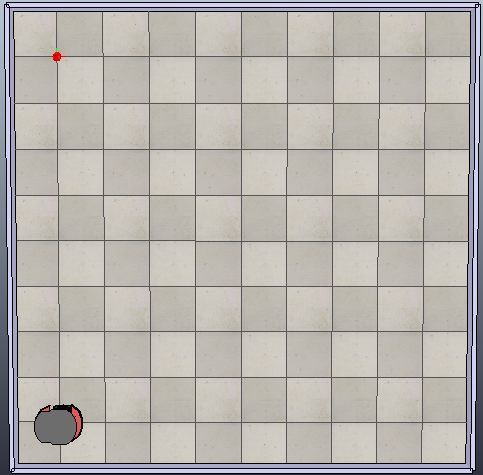
\includegraphics[width=0.3\textwidth]{Figuras/Cena_teste_2.png}
    \caption{Cena de teste 2}
    \label{fig:Cena_teste_2}
\end{figure}

\begin{figure}[h!]
    \centering
    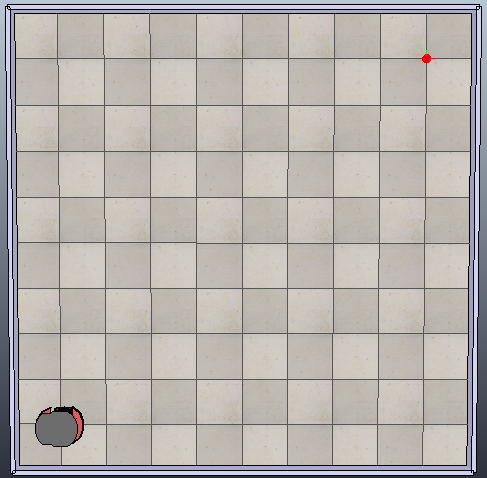
\includegraphics[width=0.3\textwidth]{Figuras/Cena_teste_3.png}
    \caption{Cena de teste 3}
    \label{fig:Cena_teste_3}
\end{figure}

\begin{figure}[h!]
    \centering
    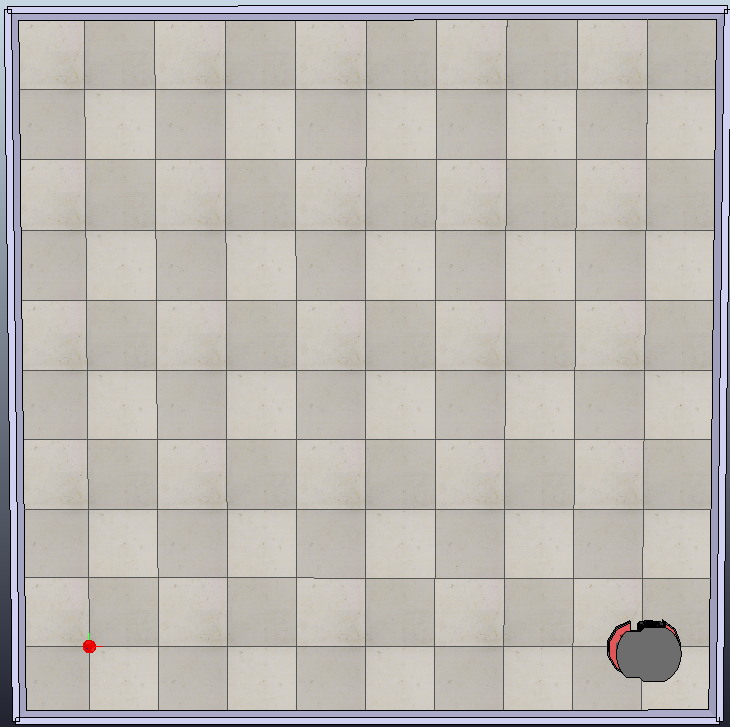
\includegraphics[width=0.3\textwidth]{Figuras/Cena_teste_4.png}
    \caption{Cena de teste 4}
    \label{fig:Cena_teste_4}
\end{figure}

Nas cenas 1, 2 e 3, o robô parte da posição inicial $(x, y) = (-2, -2)$, com orientação $\theta = 0$, entretanto, na cena 4, o robô parte da posição inicial $(x, y) = (2, -2)$, mas ainda com orientação $\theta = 0$ . Já O alvo, por sua vez, ocupa posições distintas em cada cena, tendo posições de $(2, -2)$, $(-2, 2)$, $(2, 2)$ e $(-2, -2)$ para as cenas 1, 2, 3 e 4, respectivamente.

Essas configurações permitem avaliar o comportamento do sistema de controle em diferentes situações:

\begin{itemize}
    \item Cena 1: Alvo diretamente à frente do robô;
    \item Cena 2: Alvo ao lado do robô;
    \item Cena 3: Alvo em uma posição diagonal em relação ao robô;
    \item Cena 3: Alvo diretamente atrás ao robô.
\end{itemize}

Além disso, como discutido na seção anterior, alguns parâmetros de controle precisam ser definidos para a implementação das leis de controle. No caso da abordagem de Aicardi \textit{et al.}, utilizam-se os parâmetros $\gamma$, $k$ e $h$, enquanto que na abordagem de Benbouabdallah \textit{et al.}, são empregados os parâmetros $K_v$ e $K_w$.

Considerando que qualquer valor positivo desses parâmetros satisfaz as condições de estabilidade de Lyapunov apresentadas anteriormente, e que o escopo deste trabalho não contempla a sintonização precisa desses valores, optou-se por defini-los de forma arbitrária, com o objetivo de demonstrar de forma sintética o comportamento do robô.

Os valores escolhidos foram:

\begin{itemize}
    \item \textbf{Abordagem de Aicardi \textit{et al.}}:
    \begin{itemize}
        \item $\gamma = 0.1$;
        \item $k = 1$;
        \item $h = 1$.
    \end{itemize}
    
    \item \textbf{Abordagem de Benbouabdallah \textit{et al.}}:
    \begin{itemize}
        \item $K_v = 0.1$;
        \item $K_w = 1$.
    \end{itemize}
\end{itemize}

%===================================================================================
\subsection{Resultados da Simulação}

Durante as simulações, diversas grandezas foram analisadas com maior atenção, visando avaliar a eficácia e a eficiência das leis de controle desenvolvidas.

A primeira grandeza observada foi a trajetória do robô no ambiente simulado. As Figuras~\ref{fig:Tragetória_Cena_1}, \ref{fig:Tragetória_Cena_2}, \ref{fig:Tragetória_Cena_3} e \ref{fig:Tragetória_Cena_4} ilustram o percurso do robô em cada uma das cenas, de acordo com as diferentes abordagens de controle implementadas.

\begin{figure}[h!]
    \centering
    \includegraphics[width=0.4\textwidth]{Figuras/Tragetória_Cena_1.png}
    \caption{Trajetória do robô - Cena 1}
    \label{fig:Tragetória_Cena_1}
\end{figure}

\begin{figure}[h!]
    \centering
    \includegraphics[width=0.4\textwidth]{Figuras/Tragetória_Cena_2.png}
    \caption{Trajetória do robô - Cena 2}
    \label{fig:Tragetória_Cena_2}
\end{figure}

\begin{figure}[h!]
    \centering
    \includegraphics[width=0.4\textwidth]{Figuras/Tragetória_Cena_3.png}
    \caption{Trajetória do robô - Cena 3}
    \label{fig:Tragetória_Cena_3}
\end{figure}

\begin{figure}[h!]
    \centering
    \includegraphics[width=0.4\textwidth]{Figuras/Tragetória_Cena_4.png}
    \caption{Trajetória do robô - Cena 4}
    \label{fig:Tragetória_Cena_4}
\end{figure}

Para fornecer uma noção temporal da movimentação, triângulos indicativos da posição e orientação do robô foram inseridos ao longo da trajetória, com intervalos de 1,5 segundos.

Outra grandeza monitorada foram os comandos de controle linear ($v$) e angular ($w$) ao longo do tempo. As Figuras~\ref{fig:Controle_Cena_1} a~\ref{fig:Controle_Cena_4} apresentam a evolução desses comandos em cada uma das cenas de teste.

\begin{figure}[h!]
    \centering
    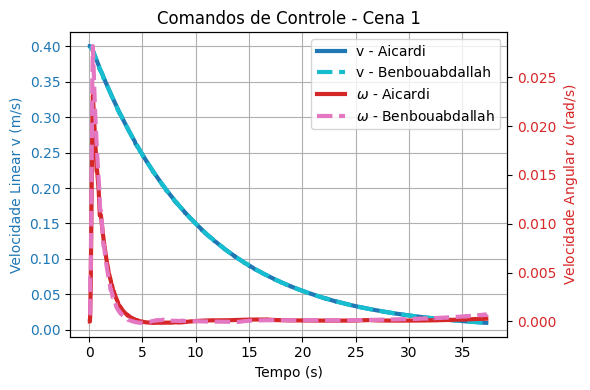
\includegraphics[width=0.4\textwidth]{Figuras/Controle_Cena_1.png}
    \caption{Comandos de controle $v$ e $w$ - Cena 1}
    \label{fig:Controle_Cena_1}
\end{figure}

\begin{figure}[h!]
    \centering
    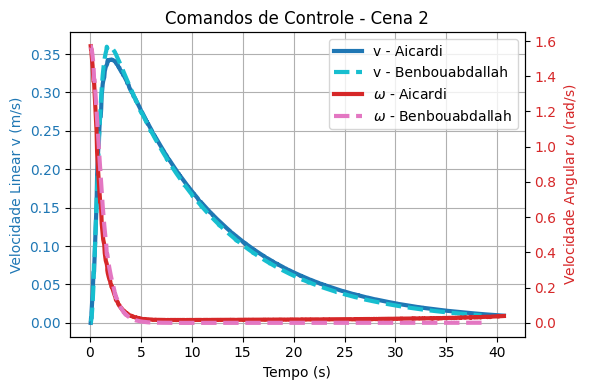
\includegraphics[width=0.4\textwidth]{Figuras/Controle_Cena_2.png}
    \caption{Comandos de controle $v$ e $w$ - Cena 2}
    \label{fig:Controle_Cena_2}
\end{figure}

\begin{figure}[h!]
    \centering
    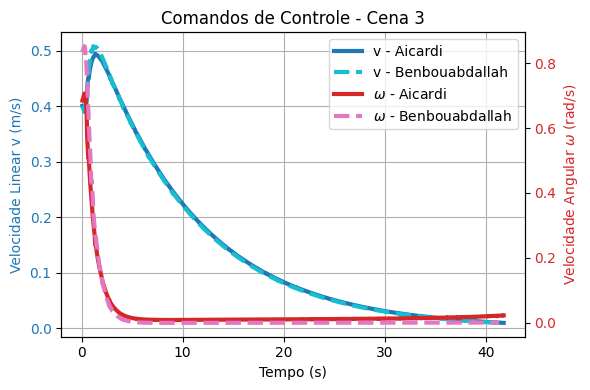
\includegraphics[width=0.4\textwidth]{Figuras/Controle_Cena_3.png}
    \caption{Comandos de controle $v$ e $w$ - Cena 3}
    \label{fig:Controle_Cena_3}
\end{figure}

\begin{figure}[h!]
    \centering
    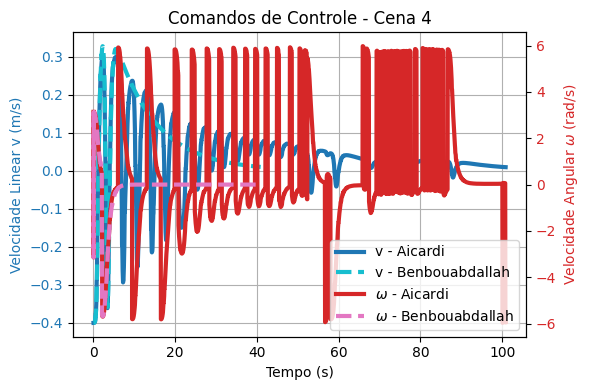
\includegraphics[width=0.4\textwidth]{Figuras/Controle_Cena_4.png}
    \caption{Comandos de controle $v$ e $w$ - Cena 4}
    \label{fig:Controle_Cena_4}
\end{figure}

Também foi analisada a distância entre o robô e o alvo, representando o erro de posição. As Figuras~\ref{fig:ErroPosição_Cena_1} a~\ref{fig:ErroPosição_Cena_4} mostram como esse erro evolui ao longo do tempo para cada cena.

\begin{figure}[h!]
    \centering
    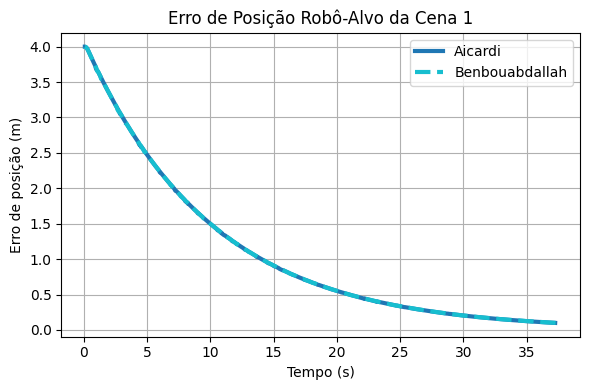
\includegraphics[width=0.4\textwidth]{Figuras/ErroPosição_Cena_1.png}
    \caption{Erro de posição - Cena 1}
    \label{fig:ErroPosição_Cena_1}
\end{figure}

\begin{figure}[h!]
    \centering
    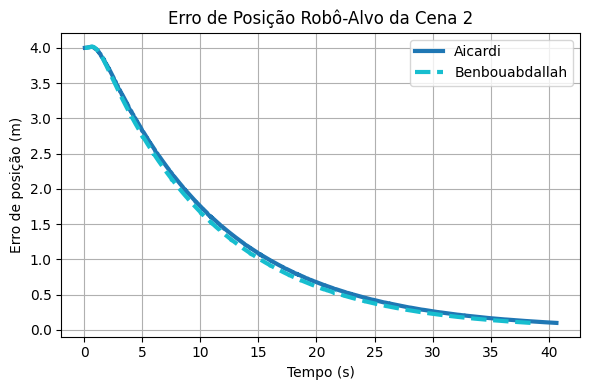
\includegraphics[width=0.4\textwidth]{Figuras/ErroPosição_Cena_2.png}
    \caption{Erro de posição - Cena 2}
    \label{fig:ErroPosição_Cena_2}
\end{figure}

\begin{figure}[h!]
    \centering
    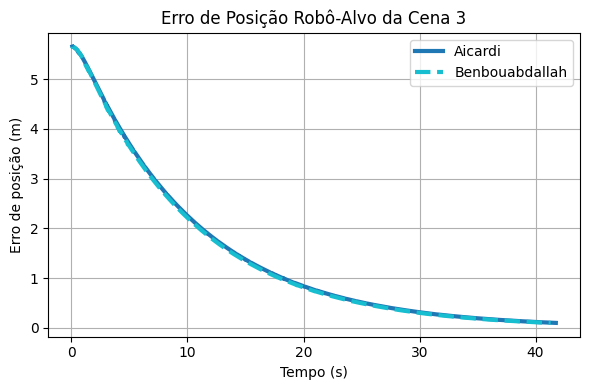
\includegraphics[width=0.4\textwidth]{Figuras/ErroPosição_Cena_3.png}
    \caption{Erro de posição - Cena 3}
    \label{fig:ErroPosição_Cena_3}
\end{figure}

\begin{figure}[h!]
    \centering
    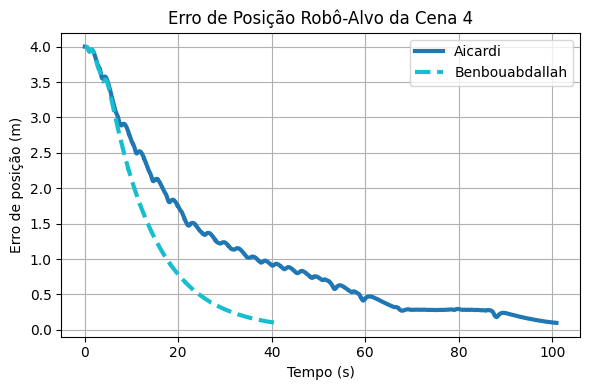
\includegraphics[width=0.4\textwidth]{Figuras/ErroPosição_Cena_4.png}
    \caption{Erro de posição - Cena 4}
    \label{fig:ErroPosição_Cena_4}
\end{figure}

Por fim, a última grandeza analisada foi o erro de orientação, representado pela variável $\alpha$. As Figuras~\ref{fig:ErroOrientação_Cena_1} a~\ref{fig:ErroOrientação_Cena_4} apresentam a evolução desse erro para cada cenário.

\begin{figure}[h!]
    \centering
    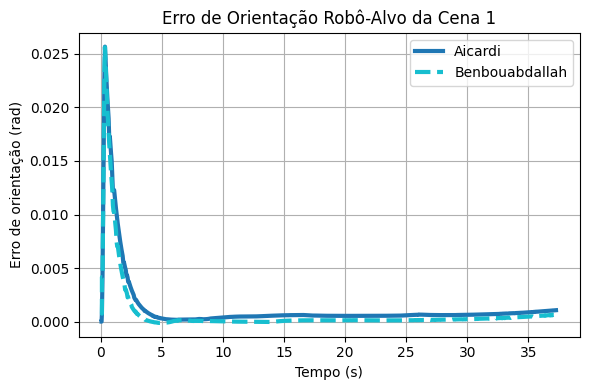
\includegraphics[width=0.4\textwidth]{Figuras/ErroOrientação_Cena_1.png}
    \caption{Erro de orientação $\alpha$ - Cena 1}
    \label{fig:ErroOrientação_Cena_1}
\end{figure}

\begin{figure}[h!]
    \centering
    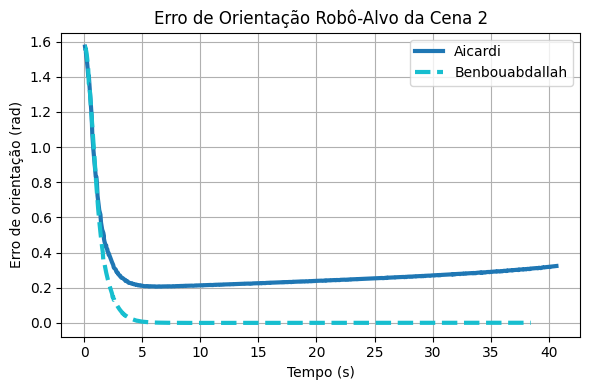
\includegraphics[width=0.4\textwidth]{Figuras/ErroOrientação_Cena_2.png}
    \caption{Erro de orientação $\alpha$ - Cena 2}
    \label{fig:ErroOrientação_Cena_2}
\end{figure}

\begin{figure}[h!]
    \centering
    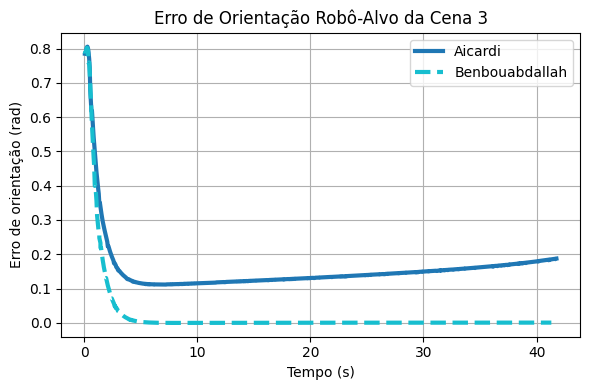
\includegraphics[width=0.4\textwidth]{Figuras/ErroOrientação_Cena_3.png}
    \caption{Erro de orientação $\alpha$ - Cena 3}
    \label{fig:ErroOrientação_Cena_3}
\end{figure}

\begin{figure}[h!]
    \centering
    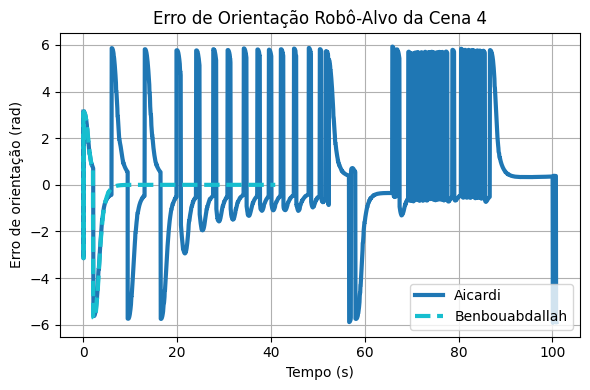
\includegraphics[width=0.4\textwidth]{Figuras/ErroOrientação_Cena_4.png}
    \caption{Erro de orientação $\alpha$ - Cena 4}
    \label{fig:ErroOrientação_Cena_4}
\end{figure}

Além dessas análises, foi calculado o tempo necessário para que o robô atingisse o alvo em cada uma das cenas. Os resultados estão organizados na Tabela~\ref{tab:Tabela_Comparacao_Tempo}, permitindo uma comparação direta entre as abordagens adotadas.

\begin{table}[h!]
    \centering
    \caption{Tempo necessário para o robô alcançar o alvo}
    \label{tab:Tabela_Comparacao_Tempo}
    \begin{tabular}{|c|c|c|c|c|}
        \hline
        \textbf{Abordagem} & \textbf{Cena 1} & \textbf{Cena 2} & \textbf{Cena 3} & \textbf{Cena 4}\\
        \hline
        Aicardi \textit{et al.} & 37.25~s & 40.65~s & 41.75~s & 100.85\\
        \hline
        Benbouabdallah \textit{et al.} & 37.35~s & 38.45~s & 41.30~s & 40.95\\
        \hline
    \end{tabular}
\end{table}

%===================================================================================
\section{Conclusão}

Os resultados das simulações demonstram que, em todos os cenários analisados, o robô foi capaz de alcançar o alvo, evidenciando que ambas as leis de controle são eficazes para resolver o problema \textit{Go-to-Goal}.

No entanto, ao se realizar uma análise comparativa entre as abordagens, observa-se que a proposta de Benbouabdallah \textit{et al.} apresenta um desempenho superior. Essa constatação pode ser verificada por meio das figuras de trajetória, erro de posição e erro de orientação, que mostram que essa abordagem permite ao robô traçar uma rota mais direta até o alvo, além de garantir um erro de orientação próximo de zero — o que indica que o robô se alinha completamente com o alvo ao final do movimento.

Destaca-se, ainda, o comportamento observado na Cena 4, em que o alvo está posicionado atrás do robô. Nesse caso, a abordagem de Aicardi \textit{et al.} encontra dificuldades significativas para alcançar o destino, ao passo que a abordagem de Benbouabdallah \textit{et al.} supera essa limitação com eficiência.

Complementarmente, a Tabela~\ref{tab:Tabela_Comparacao_Tempo} fornece uma análise quantitativa dos tempos de chegada, reforçando o desempenho superior da abordagem de Benbouabdallah \textit{et al.}, que apresenta menor tempo de conclusão na maioria das cenas, exceto na primeira, em que a diferença é mínima.

Diante dos resultados obtidos, conclui-se que a abordagem de Benbouabdallah \textit{et al.} se destaca em termos de desempenho para os parâmetros e o cenário considerados neste trabalho.


%===================================================================================

\begin{thebibliography}{00}
\bibitem{b1} AICARDI, Michele; CASALINO, Giuseppe; BICCHI, Antonio; BALESTRINO, Alberto. Closed loop steering of unicycle-like vehicles via Lyapunov techniques. IEEE Robotics \& Automation Magazine, v. 2, n. 1, p. 27–35, mar. 1995.

\bibitem{b2} BENBOUABDALLAH, Karim; ZHU, Qi-dan. A behavior-based controller for a mobile robot tracking a moving target in multi-obstacles environment. In: INTERNATIONAL CONFERENCE ON INTELLIGENT HUMAN-MACHINE SYSTEMS AND CYBERNETICS, 5., 2013, Hangzhou. Proceedings [...]. Los Alamitos: IEEE, 2013. p. 416-422. DOI: 10.1109/IHMSC.2013.247.
\end{thebibliography}

\end{document}
